% ------------------------------------------------------------------------------------
% Instruções de compilação para gerar glossário
% ------------------------------------------------------------------------------------
% pdflatex
% bibtex
% makeglossaries
% pdflatex
% pdflatex
% ------------------------------------------------------------------------------------

% ------------------------------------------------------------------------------------
% 2017-04-13 - Emerson Ribeiro de Mello - mello@ifsc.edu.br
% ------------------------------------------------------------------------------------
\documentclass[11pt]{report}
\usepackage[a4paper,hmargin=2.2cm,top=2cm,bottom=2cm]{geometry}
\usepackage{estilo-relatorio-report}
\usepackage[alf]{abntex2cite}	% Citações padrão ABNT


% Esse pacote só foi usado para gerar blocos de textos "lorem ipsum" para preencher o exemplo.
\usepackage{lipsum}


% ------------------------------------------------------------------------------------
% Definição do cabeçalho e rodapé
% ------------------------------------------------------------------------------------
\setlength{\headheight}{15pt}
\fancyhead{}
\fancyfoot{}
\renewcommand{\headrulewidth}{0pt}
\renewcommand{\footrulewidth}{0pt}

%\fancyhead[L]{ {\tiny\textsc{IFSC - Campus São José}}}
%\fancyhead[R]{ {\tiny\textsc{}}}


\fancyfoot[L]{ {\tiny\textsc{IFSC - Campus São José}}}
\fancyfoot[R]{ {\small \thepage~de~\pageref{LastPage}}}
% ------------------------------------------------------------------------------------


\makeglossaries

\begin{document}

% ------------------------------------------------------------------------------------
% Arquivo glossario.tex tem as entradas para o glossário e acrônimos
% ------------------------------------------------------------------------------------
% Os exemplos daqui foram extraídos da página https://en.wikibooks.org/wiki/LaTeX/Glossary e também de um documento de exemplo do pacote abnTeX2

% exemplo de acrônimos
\newacronym[longplural={\textit{Frames per Second}}]{fps}{FPS}{\textit{Frame per Second}}


\newglossaryentry{Linux}
{
  name=Linux,
  description={is a generic term referring to the family of Unix-like computer operating systems that use the Linux kernel},
  plural=Linuces
}

\newglossaryentry{pi}
{
  name={\ensuremath{\pi}},
  description={ratio of circumference of circle to its
               diameter},
  sort=pi
}

\newglossaryentry{numero real}
{
  name={número real},
  description={include both rational numbers, such as $42$ and 
               $\frac{-23}{129}$, and irrational numbers, 
               such as $\pi$ and the square root of two; or,
               a real number can be given by an infinite decimal
               representation, such as $2.4871773339\ldots$ where
               the digits continue in some way; or, the real
               numbers may be thought of as points on an infinitely
               long number line},
  symbol={\ensuremath{\mathbb{R}}}
}

\newglossaryentry{pai}{
                name={pai},
                plural={pai},
                description={este é uma entrada pai, que possui outras
                subentradas.} }

 \newglossaryentry{componente}{
                name={componente},
                plural={componentes},
                parent=pai,
                description={descrição da entrada componente.} }
 
 \newglossaryentry{filho}{
                name={filho},
                plural={filhos},
                parent=pai,
                description={isto é uma entrada filha da entrada de nome
                \gls{pai}. Trata-se de uma entrada irmã da entrada
                \gls{componente}.} }
 
\newglossaryentry{equilibrio}{
                name={equilíbrio da configuração},
                see=[veja também]{componente},
                description={consistência entre os \glspl{componente}}
                }

\newglossaryentry{latex}{
                name={LaTeX},
                description={ferramenta de computador para autoria de
                documentos criada por D. E. Knuth} }

\newglossaryentry{abntex2}{
                name={abnTeX2},
                see=latex,
                description={suíte para LaTeX que atende os requisitos das
                normas da ABNT para elaboração de documentos técnicos e científicos brasileiros} }
\pagestyle{empty}


% ------------------------------------------------------------------------------------
% Capa
% ------------------------------------------------------------------------------------
\begin{center}

% Logotipo do órgão

\includegraphics[scale=.7]{figuras/ifsc-logo-v}
\vspace{8cm}

% Título
{\huge \bfseries Relatório de Análise de Requisitos}

\vspace{.5cm}

% Subtítulo
{\large \bfseries Um modelo \LaTeX que faz uso da classe \texttt{report}}

\vfill

{\large \bfseries Emerson Ribeiro de Mello}

\end{center}
% ------------------------------------------------------------------------------------


% ------------------------------------------------------------------------------------
% Início do documento
% ------------------------------------------------------------------------------------
\clearpage

\section*{Histórico de revisões}
\noindent
      \begin{tabular}{|c|c|p{12cm}|} \hline
         \textbf{Data} & \textbf{Versão} & \textbf{Descrição} \\ \hline \hline
         06/11/2018 & 1.1 & Remoção das instruções para o Arara e uso da família de fontes Helvetica \\ \hline
         13/04/2017 & 1.0 & Versão inicial \\ \hline
      \end{tabular}

\clearpage


% Adicionando sumário
\tableofcontents
\printglossaries
\clearpage
\pagestyle{fancyplain}



% ------------------------------------------------------------------------------------
% Início da parte textual
% ------------------------------------------------------------------------------------

\chapter{Introdução}
\label{cap:introducao}


%% Descomente as linhas abaixo caso deseje ver como funciona a geração de glossário e lista de siglas

%Nesse modelo de relatório é feito uso do pacote \texttt{glossary} para demonstrar como fazer um glossário e uma lista de acrônimos com ele. Por exemplo, o computador precisa de um sistema de operacional e o \gls{Linux} é um bom exemplo de sistema operacional. Placa de vídeo e processador de um computador influenciam o número de quadros por segundo (\acrfull{fps}). O \gls{pi}  é um \gls{numero real}.
%
%Esse parágrafo foi obtido do modelo da classe \gls{abntex2}.  Esta frase usa a palavra \gls{componente} e o plural de \glspl{filho}, ambas definidas no glossário como filhas da entrada \gls{pai}. \Gls{equilibrio} exemplifica o uso de um termo no início da frase. O software \gls{abntex2} é escrito em \gls{latex}, que é definido no glossário como \emph{`\glsdesc*{latex}'}.
%
%Para compilar esse modelo de relatório com glossário use:
%
%\begin{verbatim}
%   pdflatex relatorio-report
%   makeglossaries relatorio-report
%   pdflatex relatorio-report
%   pdflatex relatorio-report
%\end{verbatim}

Na introdução é apresentada a organização do documento e uma breve descrição de como o mesmo foi construído.   Esse é um modelo em \LaTeX \cite{lamport94} e o estilo das referências bibliográficas segue as normas da ABNT, implementadas pelo pacote abnTeX2.

\lipsum[3]

\section{Escopo do projeto}
\label{sec:escopo}

Indica o propósito do sistema a ser desenvolvido. Por exemplo, descreve a necessidade que foi apresentada pela área requisitante. \lipsum[2]


\chapter{Requisitos do sistema}

Na \autoref{tab:pessoas} é apresentada a lista de pessoas que participaram do levantamento de requisitos. Os exemplos a seguir foram retirados de \cite{bezerra02}.

\begin{table}[!htpb]
\caption{Pessoas que participaram do levantamento de requisitos}
\label{tab:pessoas}
\begin{center}
\begin{tabular}{|l|l|l|}\hline
\textbf{Entrevistado} & \textbf{Cargo} & \textbf{Setor} \\\hline\hline
Fulano da Silva & Diretor de Ensino & Direção de Ensino\\\hline
\end{tabular}
\end{center}
\end{table}


\section{Requisitos funcionais}

\begin{enumerate}
	\item O sistema deve permitir que alunos visualizem as notas obtidas
	\item O sistema deve permitir que os alunos façam matrícula nas disciplinas do semestre letivo
	\item O sistema deve permitir que os alunos possam obter seus históricos escolares
\end{enumerate}

\section{Requisitos não funcionais}

\begin{enumerate}
	\item A interface do usuário deve ser simplificada e evitar múltiplos cliques (passos) para chegar em qualquer funcionalidade
	\item Fazer uso de protocolos criptográficos para troca de mensagens
	\item O sistema deverá ser desenvolvido em uma linguagem para web e que não dependa de plugins para o navegador
	\item O banco de dados precisar ser o MySQL
\end{enumerate}

\section{Regras de negócio}

\begin{enumerate}
	\item \textbf{Número máximo de matrículas por semestre letivo}
	\begin{itemize}
		\item Em um semestre letivo um aluno não poderá se matricular em um número de disciplinas cujo o soma de créditos ultrapasse 18.
	\end{itemize}
	\item \textbf{Número máximo de alunos por turma}
	\begin{itemize}
		\item Uma oferta de disciplina não pode ter mais de 40 vagas para matrícula.
	\end{itemize}
	\item \textbf{Validação de créditos}
	\begin{itemize}
		\item Um aluno só poderá solicitar validação de uma disciplina caso nunca tenha se matriculado na mesma.
	\end{itemize}
\end{enumerate}

\section{Casos de uso}

% Criando um contador para usar no texto exemplo desse documento
\newcounter{uc}
\newcommand{\casodeuso}{\refstepcounter{uc}UC.\arabic{uc}}


\noindent\textbf{Caso de uso:} \casodeuso~-- Realiza saque

\noindent\textbf{Ator primário:} Cliente

\noindent\textbf{Resumo: } Realizar o saque de dinheiro no terminal de atendimento

\noindent\textbf{Fluxo principal} 
\begin{enumerate}
	\item Cliente insere seu cartão no caixa eletrônico
	\item Sistema apresenta solicitação de senha
	\item Cliente digita a senha
	\item Sistema exibe menu de operações disponíveis
	\item Cliente indica que deseja realizar um saque
	\item Sistema requisita quantia a ser sacada
	\item Cliente retira o dinheiro
\end{enumerate}

\noindent\textbf{Exceções}
\begin{enumerate}
	\item Foi informada senha incorreta. Veja o caso de uso ``UC.2 -- Validar senha''
\end{enumerate}


\subsection{Matriz de rastreabilidade}

\noindent\begin{tabular}{|l|l|}\hline
\textbf{Caso de uso} & \textbf{Requisitos funcionais relacionados}\\\hline
UC.1 & R.1 e R.2\\\hline
\end{tabular}

\clearpage
\subsection{Diagrama de caso de uso}

\begin{figure}[!htbp]
	\centering
	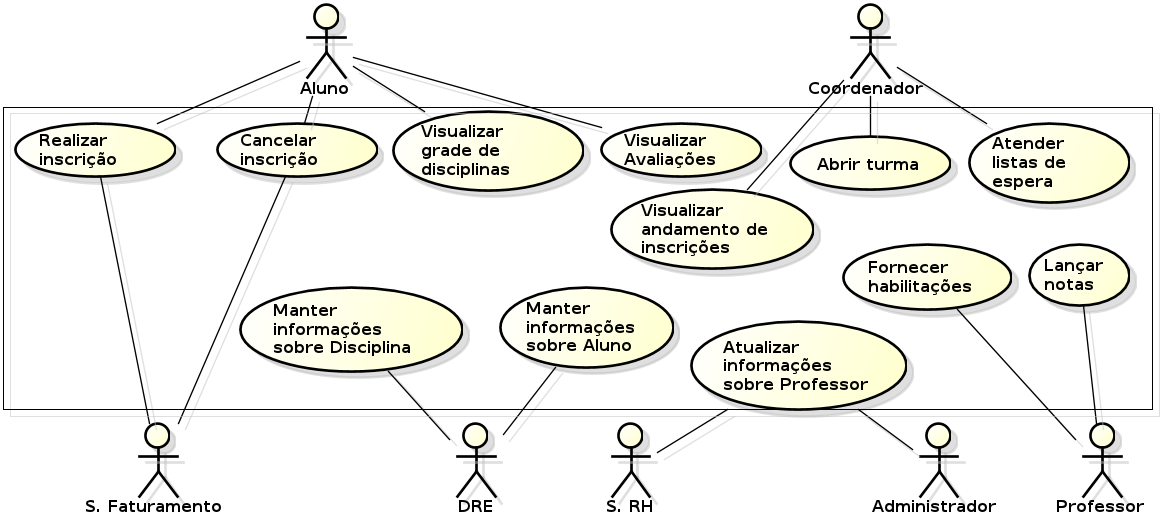
\includegraphics[width=\linewidth]{figuras/sist-acad}
	\caption{Diagrama de caso de uso do sistema acadêmico}
	\label{fig:usecase}
\end{figure}





% ----------------------------------------------------------
% Referências bibliográficas
% ----------------------------------------------------------
\bibliography{referencias}




\end{document}
